%Wir verwenden eine DIN-A4-Seite und die Schriftgröße 12.
\documentclass[a4paper,12pt]{scrartcl} 


%Diese drei Pakete benötigen wir für die Umlaute, Deutsche Silbentrennung etc.
%Apple-Nutzer sollten anstelle von \usepackage[latin1]{inputenc} das Paket \usepackage[applemac]{inputenc} verwenden
%% \usepackage[latin1]{inputenc}
%%apt-get install texlive-lang-german damit ngerman keine Probleme mehr macht !!
%\usepackage[utf8]{inputenc} 
%\usepackage[T1]{fontenc}
%\usepackage[ngerman]{babel}

%Das Paket erzeugt ein anklickbares Verzeichnis in der PDF-Datei.
%\usepackage{hyperref}

%Das Paket wird für die anderthalb-zeiligen Zeilenabstand benötigt
\usepackage{setspace}

%%HTWM-Vorlage - benoetigt apt-get install texlive-fonts-extra
\setcounter{tocdepth}{3}				%Schatelungstiefe Inhaltsverz.
\usepackage[utf8]{inputenc}			%deutsche Umlaute
\usepackage[ngerman]{babel}			%Rechtschreibprüfung
\usepackage{color,listings} 			%Quellcode Highlighting, bindet das
%Paket Listings ein
\usepackage{listings}
\usepackage{color}
\usepackage{textcomp}
\usepackage[T1]{fontenc}				%srccode
\usepackage[scaled]{beramono}		%srccode
\usepackage{longtable}				%mehrseitige tabellen
\usepackage[tableposition=b]{caption}
\usepackage[pdftex, pdftoolbar=false, hyperfootnotes=false, bookmarks,
bookmarksopen, bookmarksnumbered, bookmarksopenlevel=2, pdfpagelabels=true,
pdfstartpage=3, pdfstartview=FitH,]{hyperref} %Verlinkungen
\usepackage{array}					%farbige Tabellen
\usepackage[table]{xcolor} 			%farbige Tabellen
\usepackage{graphicx}				% \includegraphics bnoetigt dies
\usepackage{draftwatermark}			% wasserzeichen
	%Quelle: http://choorucode.com/2010/05/05/latex-adding-draft-watermark/?like=1&source=post_flair&_wpnonce=1c9f85538d
\SetWatermarkText{VORABVERSION}		% wasserzeichen-text
\SetWatermarkLightness{0.9}			% wasserzeichen-kontrast
\SetWatermarkScale{2.5}				% wasserzeichen-zeichengroe\ss{}e

\newcommand{\includesvg}[1]{
\immediate\write18{inkscape -z -D –file=images/#1.svg
–export-pdf=images/#1.pdf –export-latex}
\input{images/#1.pdf_tex}
}

\definecolor{Navy}{rgb}{0,0,0.5}
\definecolor{Gray}{gray}{0.5}
\definecolor{dunkelgrau}{rgb}{0.8,0.8,0.8}
\definecolor{hellgrau}{rgb}{0.95,0.95,0.95}
\definecolor{hellgrau2}{rgb}{0.93,0.93,0.93}

\hypersetup{
	colorlinks=true, 			% false: boxed links; true: colored links
	linkcolor=Navy,          		% color of internal links
	citecolor=Gray,        			% color of links to bibliography
	filecolor=magenta,      		% color of file links
	urlcolor=blue,           			% color of external links
	linkbordercolor={1 1 1}, 		% set to white
	citebordercolor={1 1 1} 		% set to white
}


%Einrückung eines neuen Absatzes
\setlength{\parindent}{0em}

%Definition der Ränder
\usepackage[paper=a4paper,left=30mm,right=30mm,top=30mm,bottom=30mm]{geometry} 

%Abstand der Fussnoten
\deffootnote{1em}{1em}{\textsuperscript{\thefootnotemark\ }}

%Regeln, bis zu welcher Tiefe (section,subsection,subsubsection) Überschriften angezeigt werden sollen (Anzeige der Überschriften im Verzeichnis / Anzeige der Nummerierung)
%\setcounter{tocdepth}{3}
%\setcounter{secnumdepth}{3}



\begin{document}

%Beginn der Titelseite
\begin{titlepage}
\begin{small}
\vfill {HTWK Leipzig\\ 
Fachbereich IMN \\ 
Wintersemester 2012/2013}
\end{small}


\begin{center}
\begin{Large}
\vfill {\textsf{\textbf{
Die Möglichkeiten des System-Managements der Firewall-Distribution
pfSense\\--VORABVERSION--\\
}}}
\end{Large}
Beleg im Fach Netzwerk- und System-Management
\end{center}

\begin{small}
\vfill Marcel Kirbst \\ Sieglitz 39 \\  06618 Molau \\
marcel.kirbst@stud.htwk-leipzig.de\\
\today
\end{small}

\end{titlepage}
%Ende der Titelseite


%Inhaltsverzeichnis (aktualisiert sich erst nach dem zweiten Setzen)
\tableofcontents
\thispagestyle{empty}

%Beginn einer neuen Seite
\clearpage

%Anderthalbzeiliger Zeilenabstand ab hier
\onehalfspacing

\pagestyle{plain}


\section{Einleitung}
Dieser Beleg befasst sich der Vorstellung der Routerdistribution pfSense.
Im Vergleich zu den unzähligen anderen, existierenden Routerdistributionen
zeichnet sich pfSense durch seinen hohen Funktionsumfang aus, der beispielsweise
auch Funktionen zur Sicherstellung von Redundanz und Ausfallsicherheit umfasst,
wie sie sonst nur bei preisintensiven proprietären Lösungen kommerzieller
Anbieter verfügbar sind.


Nachdem grundlegende Begriffe erläutert wurden, soll kurz auf die
Entwicklungsgeschichte und Vorzüge des Betriebssystems FreeBSD eingegangen
werden, welches die Grundlage für pfSense bildet. Im folgenden soll ein kurzer
Überblick über den Funktionsumfang von pfSense gegeben werden, für sich genommen
und im Vergleich zu anderen Rouuterdistributionen. Abschließend sollen
beispielhaft drei Konfigurationen vorgestellt werden um die Vielseitigkeit und
Leistungsfähigkeit von pfSense zu demonstrieren.

%\begin{figure}[htb]
%  \begin{center}
%    \includegraphics[width=1\hsize]{./images/test.png}
%  \end{center}
%  \caption[PNG-File]{\label{Test-Import: PNG-File} Test-Import PNG-FIle}
%\end{figure}

%\begin{figure}
%\centering
%% \def\svgwidth{\columnwidth}
%\includesvg{./images/default}
%\end{figure}

\begin{center}
 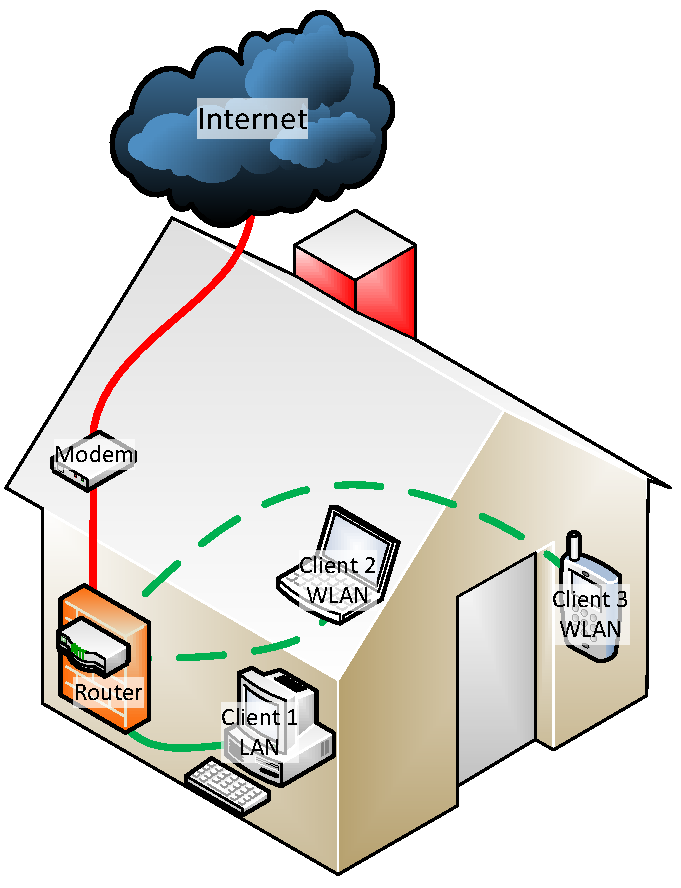
\includegraphics[width=2\hsize]{./images/default.pdf}
 % test.pdf: 595x842 pixel, 72dpi, 20.99x29.70 cm, bb=0 0 595 842
\end{center}


\section{Routerdistributionen - Besonderheiten und Merkmale im Allgemeinen}

\subsection{Begrifflichkeiten im Zusammenhang mit Routerdistributionen}
Routerdistributionen sind auf einen speziellen Einsatzzweck hin optimierte
Betriebssysteme.

Unter dem Begriff Betriebssystem fasst man eine Menge von Software zusammen, die
auf einem Rechnersystem nach dem Start zur Ausführung kommt, die Ressourcen
dieses Rechnersystems verwaltet und es ermöglicht weitere Anwenungsprogramme zu
starten.

Routerdistributionen werden in der Regel so konzipiert und entwickelt,
um direkt auf einem Rechnersystem installiert zu werden und über alle Ressourcen
dieses Rechnersystems zu verfügen. Dieser Annahme kommt eine besonders hohe
Bedeutung zu, da die beiden Schwerpunkte einer Routerdistribution Sicherheit und
Stabilität darstellen. Andere Merkmale wie zum Beispiel m\"oglichst hoher
Funktionsumfang besitzen dem gegen\"uber niedrigere Priorit\"at, wobei jedoch
verschiedene Routerdistributionen die einzelnen Merkmale im
Detail unterschiedlich stark priorisieren.

Ein Router ist ein Netzwerkgerät, das mit mindestens zwei
Netzwerkschnittstellen ausgestattet ist und den Netzwerkverkehr zwischen den
betreffenden Netzwerken, unter Beachtung eines vorgegebenen Regelwerkes,
vermittelt.

\subsection{Merkmale von Routerdistributionen}
Routerdistributionen werden in der Regel nicht von Grund auf entwickelt sondern
basieren auf einem modifizierten Betriebssystem. Trotz dieser Modifikationen
unterliegen die verschiedenen Routerdistributionen somit mehr oder weniger
stark den Merkmalen, Besonderheiten und Einschr\"ankungen des jeweils zu Grunde
liegenden Betriebssystems. Somit ist das zu Grunde liegende Betreibssystem ein
erstes wichtiges Unterscheidungskriterium f\"ur Routerdistributionen.

Ein weiteres wichtiges Unterscheidungskriterium stellt die Art der Entwicklung
und Lizenzierung dar. Es existieren kommerzielle Produkte genauso wie
quelloffene Produkte. Da kommerzielle Produkte in den allermeisten F\"alle
jedoch nicht im Quellcode verf\"ugbar und somit schwer an spezielle
Bed\"urfnisse anzupassen sind und au\ss{}erdem oft betr\"achtliche Lizenzkosten
verursachen, soll dieser Typus von Routerdistributionen in dieser Arbeit
au\ss{}en vor bleiben. 
 
Weiterhin spielt f\"ur den potentiellen Einsatz im kommerziellen Umfeld
neben Funktionen wie zum Beispiel VLAN-Unterst\"utzung auch der Faktor der
Verf\"ugbarkeit eines kommerziellen Supports eine wichtige Rolle. Steht f\"ur
komplexe Netzwerke wie etwa in Hochschulen oder mittelst\"andischen und
gro\ss{}en Unternehmen mit hunderten bis tausenden Nutzern die Konzeption und
Implementierung einer Router- und Firewalll\"osung bevor, ist es in der Regel
obligatorisch, gegebenenfalls auf schnellen kommerziellen Support
zur\"uckgreifen zu k\"onnen.

Um den generellen Kostenrahmen absch\"atzen zu k\"onnen und damit
Planungssicherheit in einem bestimmten Rahmen zu bieten, sollte au\ss{}erdem
eine Bedarfsanalyse durchgef\"uhrt werden. Diese sollte nicht nur die
derzeitigen Anforderungen ber\"ucksichtigen, sondern auch zuk\"unftige wie zum
Beispiel die vollst\"andige Unterst\"utzung von IPv6.

Au\ss{}erdem sollen die Routerdistributionen im Bezug auf modulare
Erweiterbarkeit betrachtet werden, denn bei Verf\"ugbarkeit speziell
vorgefertigter Softwarepakete, oft auch als so genannte Addons bezeichnet
werden l\"asst sich der Nutzen der Routerdistribution f\"ur den Adminsitrator
oft erheblich steigern. Jedoch soll an dieser Stelle ausdr\"ucklich darauf
hingewiesen werden, dass jeder zus\"atzliche Dienst auch zus\"atzliche
potentielle Sicherheitsl\"ucken birkt. Es gilt also im Bezug auf zus\"atzliche
Dienste bei Routerdistributionen und Firewalls der Grundsatz: ``So viel wie
n\"otig, jedoch so wenig wie m\"oglich!''
 
\subsection{Konkrete Routerdistributionen im Vergleich}
Im Folgenden soll ein Vergleich dreier verbreiteter OpenSource-
Routerdistributionen erfolgen. 

\subsubsection{Die Routerdistribution IPCop}
IPCop ist eine Router-Distribution, die auf dem Betriebssystemkern Linux
basiert und in der Version 1.0 bereits am 1. Januar 2002 ver\"offentlicht
wurde. \footnote{\cite{IPCopManual}}

Nach Aussagen der Entwickler von IPCop ist die Entwicklung vor allem auf eine
zuverl\"assige, sichere und stabile Routerdistribution hin ausgerichtet, die
auch von Laien eingerichtet und betrieben werden kann. Nach der Installation
lassen sich s\"amtliche Konfigurationsparamter \"uber eine Weboberfl\"ache
modifizieren, ein Zugriff auf die Kommandozeile der Routerdistribution ist also
im Normalfall nicht erforderlich, jedoch m\"oglich. 

Eine Erweiterbarkeit um viele Funktionen, die zu Lasten der Sicherheit geht,
steht dagegen hinten an. Als Beispiel sei an dieser Stelle das Samba-Addon f\"ur
IPCop erw\"ahnt, das es erm\"oglichte IPCop um einen Samba-Server zu erweitern,
um den Rechner im lokalen Netzwerk hinter der IPCop einen Dateiserver
haupts\"achlich f\"ur Windows-Clients zu bieten. Dieses Addon wurde absichtlich
nicht mehr verf\"ugbar gemacht um die Sicherheit der IPCop-Firewall nicht durch
diesen zus\"atzlichen Dienst herabzusetzen.\footnote{\cite{IPCopSamba}}

Mit dem Erscheinen von IPCop Version 2.0 im Jahr unterst\"utzt IPCop weitere
Hardware-Architekturen wie PowerPC, Cobalt und
Sparc. Au\ss{}erdem erfolgte mit Einf\"uhrung
von Version 2.0 eine \"Uberarbeitung
verschiedener Dienste wie zum Beispiel des
Zeitservers und des DHCP-Servers\footnote{\cite{IPCop20Hardware}}

Es l\"asst sich also sagen, dass IPCop eine Routerdistribution ist, die sich
nicht durch m\"oglichst hochgradigen Funktionsumfang sondern durch Sicherheit
und Stabilit\"at definiert. 

\subsubsection{Die Routerdistribution IPFire}
IPFire basiert wie pfSense auf dem Betriebssystemkern Linux. Im Vergleich zu
IPCop versucht man jedoch bei IPFire mehr Modularit\"at zu bieten, indem f\"ur
viele popul\"are Dienste wie Asterisk, eine Telefonserver-Software oder Samba,
vorkonfigurierte Pakete zur Verf\"ugung stehen.

Weiterhin existieren auf der offiziellen Webpr\"asenz auch Anleitungen um
Instanzen von IPFire in einer virtuellen Umgebung wie zum Beispiel unter Xen
zur Ausf\"uhrung zu bringen.\footnote{\cite{IPFireAddons}} Die Virtualisierung
von Firewalls ist jedoch ein eigenes, umstrittenes Gebiet, dass in dieser
Arbeit nicht weiter aufgegriffen werden soll. Es wird auf entsprechende
Literatur verwiesen. (QUELLEN EINF\"UGEN !!)

Im Bezug auf IPFire ist festzuhalten, dass diese wie auch IPCop auf Linux
basiert, jedoch im Vergleich zu IPCop mehr versucht einen Kompromiss zwischen
Sicherheit und Erweiterbarkeit zu bieten.

\subsubsection{Die Routerdistribution pfSense}
Die Routerdistribution pfSense basiert auf dem Betriebssystem FreeBSD. Wie die
anderen vorgestellen Routerdistributionen l\"asst sich auch pfSense nach der
Installation quasi vollst\"andig \"uber die Weboberfl\"ache administrieren.

Da pfSense auf FreeBSD aufbaut, ist diese Routerdistribution auch den gleichen
Vorz\"ugen und Nachteilen unterworfen wie FreeBSD.

Die Hardwareunterst\"utzung von FreeBSD ist nicht so umfangreich wie
beispielsweise f\"ur Linux. Das sollte bei der Anschaffung von neuer Hardware
f\"ur Routerdistributionen beachtet werden.\footnote{\cite{FreeBSDHardware}} Im
Gegenzug bietet FreeBSD von Haus aus schon enorme Vorteile im Bezug auf den
Funktionsumfang, beispielsweise war FreeBSD eines der ersten Betriebssystem die
den IPv6-Stack vollst\"andig implementierten. Weitere Funktionen sind die
Unterst\"utzung von VLANS beim Einsatz geeigneter Netzwerkkarten sowie
Implementierung von Techniken Wie CARP und XMLRPC, die Vorraussetzung sind,
wenn redundante Router- und Firewallcluster implementiert werden sollen.

Weiterhin existiert f\"ur pfSense ein eigenes Paketverwaltungssystem, welches
direkt aus der Weboberfl\"ache erreichbar ist und die pfSense um weitere
Dienste und Funktionen erweitern kann. Es folgt eine Auflistung einer Auswahl
von Paketen:
\begin{description}
 \item[asterisk] verbreiteter Telefonserver-Dienst
 \item[country block] erlaubt das Blockieren von eingehendem Internetverkehr
anhand dessen l\"anderspezifischer Herkunft
 \item[freeradius] freie Implementierung eines Radius-Servers der es
erm\"oglicht, die Benutzer s\"amtlicher Dienste im Netzwerk gegen diesen Dienst
authentifizieren zu lassen, beispielsweise Dateiserver oder WLAN-Zugang auf
Basis von WPA(2)-Enterprise.
 \item[squid] leistungsf\"ahiger Proxy-Server.
\end{description}

Durch den hohen Funktionsumfang der auch Techniken zur Hochverf\"ugbarkeit und
logischen Segmentierung des lokalen Netzwerks umfasst ist pfSense f\"ur den
Einsatz in mittleren bis gro\ss{}en Netzwerken, wie sie in Unternehmen und
Hochschulen \"uberlicherweise vorhanden sind, eine interessante Alternative zu
kommerziellen Produkten. Jedoch ist auch im Privatbereich der Einsatz von
pfSense als Heimrouter-Software \"ublich, unter anderem deshalb, weil eine
\"ubersichtliche und gut strukturiere Weboberfl\"ache Bestandteil dieser
Routerdistribution ist, die auch mehrere Assistenen beinhaltet um dem
Administrator die Konfiguration zu erleichtern

\subsubsection{Leistungsmerkmale der vorgestellten Routerdistributionen im
Vergleich}
Im folgenden sollen die wichtigsten Vorz\"uge und Leistungsmerkmale der
ausgew\"ahlten Routerdistributionen noch einmal direkt gegen\"uber gestellt
werden.\\


Ber\"ucksichtigt werden im Folgenden jedoch nur Funktionen, die bei einer
Standardinstallation bereits verf\"ugbar sind oder durch ein eventuell
vorhandes Paketmanagement f\"ur die jeweilige Routerdistribution
benutzerfreundlich nachger\"ustet werden k\"onnen und somit die Stabilit\"at
und Sicherheit des Gesamtsystems nicht oder nur geringf\"ugig verschlechtern.
Da es sich bei allen drei Kandidaten um OpenSource-L\"osungen handelt k\"onnen
zus\"atzliche Funktionen nat\"urlich mit unterschiedlich hohem Aufand trotzdem
nachger\"ustet werden, jedoch handelt es sich dann um individuelle
Modifikationen die in der Praxis in der Regel nicht im gr\"o\ss{}eren Umfeld
getestet wurden und eventuell bei sp\"ateren Updates der Firewalldistribution
Konflikte verursachen.\\

-tabellarische Auflistung-
Betriebssystem, unterst\"utzte Hardwarearchtiketuren, eigene Paketverwaltung,
Automatisches Update, VLAN, Art und Anzahl Netzwerk-Interfaces, Redundanz\\


%\vspace*{1cm}
\begin{longtable}{p{34mm}>{\columncolor[gray]{0.97}}p{33mm}p{33mm}>{\columncolor
[gray]{0.97}}p{33mm}}
\rowcolor[gray]{.9}Funktion & \textbf{IPCop} & \textbf{IPFire} &
\textbf{pfSense}\\
Lizenz & GPL & GPL & BSD\\
\rowcolor[gray]{.95}Betriebssystem & Linux & Linux & FreeBSD   \\
Hardware"-architektur & i386, Cobald, Sparc, PowerPC & i386,
AMD64 & i386, AMD64\\
\rowcolor[gray]{.95}vorkonfigurierte Pakete & nein & ja & ja \\
eigene Paketverwaltung & nein & nein & ja \\
\rowcolor[gray]{.95}Automatisches Update & nein & nein & ja \\
VLAN-Unterst\"utzung & nein & nein & ja mit entsprechenden
Netzwerkkarten\\
\rowcolor[gray]{.95}Netzwerkschnittstellen & max. 4 & max. 4 & nur durch
Hardware begrenzt \\
\caption{Merkmale der Routerdistributionen im Vergleich}
\label{Merkmale der Routerdistributionen im Vergleich}
\end{longtable}


Auswahl und Begr\"undung einer konkreten Routerdistribution f\"ur die
beispielhafte Implementierung von Praxisf\"allen im folgenden Kapitel

\section{Ausgew\"ahlte Anwendungsf\"alle von pfSense}
In diesem Kapitel soll die Implementierung praxisnaher Anwenungsf\"alle
dokumentiert werden um die M\"oglichkeiten des Systemmanagements von pfSense
vorzustellen. 

\subsection{pfSense als DSL-Router im Heimbereich}
Hier beginnt der erste Unterabschnitt des zweiten Hauptteils.

\subsection{pfSense als redundanter Firewall-Cluster im Firmenumfeld}
Hier beginnt der zweite Unterabschnitt des zweiten Hauptteils.


\section{Schluss}
Dies ist der Schlussteil. Abschlie\ss{}ende Empfehlung
%Beginn einer neuen Seite
\clearpage

\section{Glossar}
\begin{description}
 \item[DHCP-Server] DHCP steht als Abk\"urzung f\"ur "Dynamic Host
Configuration Protokoll" und beschreibt Techniken um Hosts in Netzwerken
dynamisch Netzwerkparameter wie IP-Adressen zuzuwei\ss{}en\footnote{\cite{dhcp}}
 \item[Router] Ein Rechnersystem mit mindestens zwei Netzwerkschnittstellen,
das Netzwerkschverkehr zwischen diesen Netzwerkschnittstellen nach einem
Regelwerk vermittelt und weiterleitet.
 \item[Routerdistribution] Eine spezielle Art von Betriebssystem, deren
Hauptaugenmerk bei der Konzeption und Entwicklung darauf liegt
Router-Funktionen sicher und stabil auszuf\"uhren
 \item[VLAN] Die Abk\"urzung VLAN steht f\"ur Virtual Local Area Network und
fasst Techniken zusammen um physikale Netzwerkstrukturen logisch zu
Segmentieren, beispielsweise zur Erh\"ohung der Sicherheit oder um
Broadcast-Dom\"anen zu verkleinern.
\end{description}
\clearpage

\section{Literaturverzeichnis}

Musterfrau, Renate: Muster. Frankfurt 2003.


Mustermann, Helmut: Noch ein Muster. Mit einer Einleitung hrsg. von Frank Muster. Frankfurt 2003.

\begin{thebibliography}{99}

\bibitem{IPCopManual} http://www.ipcop.org/1.4.0/en/install/html/ , abrufbar am
16.12.2012

\bibitem{IPCopSamba} http://www.ipcopwiki.de/index.php/Samba\_Server ,
abrufbar am 20.12.2012\\
\textit{Anm.: Der Artikel zu diesem Addon ist zwar noch verf\"ugbar, jedoch
nicht die eigentlichen Dateien, die f\"ur das Addon erforderlich sind.}

\bibitem{IPCop20Hardware}
http://www.ipcop.org/2.0.0/en/admin/html/whatsnew.html , abrufbar am 11.01.2013

\bibitem{IPFireAddons} http://wiki.ipfire.org/de/addons/start , abrufbar am
10.01.2013

\bibitem{FreeBSDHardware}
http://www.freebsd.org/doc/de/books/faq/hardware.html\#which-hardware-to-get ,
abrufbar am 12.01.2013

\bibitem{dhcp} http://www.isc.org/software/dhcp , abrufbar am 11.01.2013

\end{thebibliography}
\end{document}
%% EOF